\documentclass{article} % For LaTeX2e
\usepackage{amsthm}
\usepackage{amssymb}
\usepackage{amsmath}
\usepackage{bibentry}
\usepackage{caption}
\usepackage{hyperref}
\usepackage{listings}
\usepackage{natbib}
\usepackage{tikz}
\usetikzlibrary{bayesnet}
\usepackage{wrapfig}
\usepackage{xstring}
\usepackage{url}

\usepackage{nips14submit_e}
\usepackage{times}


\title{Title}

\author{
Tal Friedman \\
\texttt{talf301@gmail.com} \\
\And
Erin Grant \\
\texttt{erin.grant@mail.utoronto.ca}
}


\newcommand{\fix}{\marginpar{FIX}}
\newcommand{\new}{\marginpar{NEW}}
\newcommand{\argmax}{\operatornamewithlimits{argmax}}

% Reference label commands
\newcommand{\Table}[1]{Table~\ref{#1}}
\newcommand{\Algorithm}[1]{Algorithm~\ref{#1}}
\newcommand{\Section}[1]{Section~\ref{#1}}
\newcommand{\Example}[1]{\ref{#1}}
\newcommand{\Figure}[1]{Figure~\ref{#1}}
\newcommand{\Equation}[1]{Eqn.~(\ref{#1})}
\newcommand{\Page}[1]{page~\pageref{#1}}


%% colour definitions
\definecolor{pink}{HTML}{F67088}
\definecolor{orange}{HTML}{CE8F31}
\definecolor{green}{HTML}{32B165}
\definecolor{blue}{HTML}{38A7D0}
\definecolor{purple}{HTML}{A38CF4}


%% tikz definitions

% bayes net nodes
\tikzstyle{item on} = [draw, circle, fill=blue!50, text centered, minimum size=3em]
\tikzstyle{item off} = [draw, circle, fill=blue!25, text centered, minimum size=3em] 
\tikzstyle{hidden on} = [draw, circle, fill=orange!50, text centered, minimum size=3em]
\tikzstyle{hidden off} = [draw, circle, fill=orange!25, text centered, minimum size=3em] 
\tikzstyle{query on} = [draw, circle, fill=purple!50, text centered, minimum size=3em]
\tikzstyle{query off} = [draw, circle, fill=purple!25, text centered, minimum size=3em] 

% ontology nodes
\tikzstyle{disease} = [draw, rectangle, rounded corners, fill=blue!25, text centered, align=center]
\tikzstyle{phenotype} = [draw, rectangle, rounded corners, fill=purple!25, text centered, align=center]

% algorithm style
\lstnewenvironment{algorithm}[1][] %defines the algorithm listing environment
{   
    \lstset{
        frame=tb,
        commentstyle=\itshape,
        numbers=left, 
        numberstyle=\tiny,
        keywordstyle=\color{black}\bfseries,
        keywords={,input, output, return, in, if, else, foreach, while, },
        xleftmargin=.04\textwidth,
        mathescape=true,
    }
}
{}


%\nipsfinalcopy % Uncomment for camera-ready version


\begin{document}

%\nobibliography*

\maketitle


\begin{abstract}

    Blah blah blah.

\end{abstract}


\section{Introduction}
\label{sec:intro}

[TODO: introduce disease diagnosis in general, reference QR network or something like that]
Computer assisted diagnosis is a useful and desirable tool that has been challenging the AI community for many years. Jaakkola et Al. \cite{qmrdt} introduced the QMR-DT network, an example of a major use of a probabilistic graphical model built on expert knowledge used for CAD. 
In particular, computer-assisted diagnosis (CAD) is useful in the realm of rare genetic diseases: clinical geneticists will often be tasked with diagnosing patients with disorders they may only see a couple of times in their careers. In this regard, having a tool which can make some reasonable suggestions for diagnoses a clinician may have never seen before is invaluable. \\
In order for a CAD system to be feasible, one requires either a very large training set of diagnosed patients, or some expert information relating disorders and symptoms. Clearly, the first option is not a possibility in our domain, but the Human Phenotype Ontology (HPO) \cite{kohler2014hpo} and OMIM \cite{omim}

% TODO: emphasise that we are talking about rare genetic diseases and not other types of diseases
\section{Previous Work}
\label{sec:lit-rev}

Bauer et al.\ \cite{bauer2012bayesian} introduced a disease diagnosis system
that uses Bayesian inference to resolve diagnostic queries, entitled the 
{\it Bayesian Ontology Query Algorithm} (BOQA).
%
The system comprises a Bayesian network with three layers of Boolean variables:
an {\it item} layer of diseases, a {\it hidden} layer of phenotypic features,
and a {\it query} layer of phenotypic features.
%
\footnote{
    In this report, we use the term {\it phenotype} interchangeably with symptom,
    since all symptoms of interest to the model are expected to have their root
    in genetic disorders.
}
%
The causal relationships between a disease and its related symptoms are modelled
as a set of directed edges from each disease node in the {\it item} layer to its
subset of phenotypic nodes in the {\it hidden} layer.
%
We may refer to the symptoms caused by a disease as the disease's {\it phenotype
annotations}.
%
Each phenotype node in the hidden layer is paired with exactly one node in the
query layer, by a directed edge from the node in the hidden layer to its
correspondent in the query layer.

We may interpret this model in a generative fashion as follows:
%
the occurrence of a disease (activity in an item node) causes its symptoms to
occur with some probability (activity in a hidden node). Furthermore, the
presence of a symptom (activity in a hidden node) may lead to the clinician
detecting the symptom (activity in a query node). However, the clinician may
fail to recognize the occurrence of a symptom (activity in a hidden node without
activity in the corresponding query node), or the clinician could perceive a
symptom where none exists (activity in a query node without
activity in the corresponding hidden node).
%
In this way, the hidden layer allows the system to model uncertainty about the
accuracy of a clinician's symptomatic description.

In addition to the edges between layers, BOQA contains within-layer connections
to model the ontology of phenotypes described by the Human Phenotype Ontology
(HPO) \cite{kohler2014hpo}.
%
Within the hidden layer, there is a directed edge from node $H_a$ to $H_b$
if the annotation of the phenotype $H_a$ to a disease implies that the phenotype
$H_b$ is also annotated to the disease.
%
Such an edge is present in the network if the phenotype $H_a$ is a child of
phenotype $H_b$ in the HPO. 
%
These edges serve the purpose of encoding the {\it annotation propagation rule}:
if an item $i$ is annotated to term $j$ then it is implicitly annotated to all
ancestors of $j$.

Lastly, in the case that the edge from $H_a$ to $H_b$ is present, then  in the
query layer, there is a directed edge from phenotype $Q_b$ to phenotype $Q_a$ (i.e., an edge in the
inverse direction of the edge $H_a \to H_b$).
%
These edges serve to encode the fact that a if a phenotype $Q_a$ is in the search query, then so are all of its ancestors.
%
\begin{center}
\begin{figure}[h]
\newcommand{\itemlayer}{$I_1$/A, $I_2$/B}
\newcommand{\hiddenquerylayers}{$H_1$/C/$Q_1$/J, $H_2$/D/$Q_2$/K, $H_3$/E/$Q_3$/L, $H_4$/F/$Q_4$/M, $H_5$/G/$Q_5$/N, $H_6$/H/$Q_6$/O, $H_7$/I/$Q_7$/P}
%
    \label{fig:bauer-net}
    \begin{tikzpicture}
        \pgfmathsetmacro\diametersqr{1}
        \pgfmathsetmacro\rectwidth{2}
        \pgfmathsetmacro\rectheight{8}
        \pgfmathsetmacro\spacing{1}
        
        \pgfmathsetmacro\numnodesitem{2}
        \pgfmathsetmacro\numnodeshiddenquery{7}
        
        % item layer
        \xdef\xlist{4}
        \xdef\ylist{4}
        \pgfmathsetmacro\yoffset{\rectheight / \numnodesitem}
        \foreach \m/\n [count=\l] in \itemlayer{
            \foreach \k in {1,...,400}{ % try 400 times to place without a collision
                \pgfmathsetmacro\x{rnd*\rectwidth}
                \pgfmathsetmacro\y{(\l - 1)*\yoffset + rnd*\yoffset}
                \xdef\collision{0}
                \foreach \element [count=\i] in \xlist{
                    \pgfmathtruncatemacro\j{\i-1}
                    \pgfmathsetmacro\checkdistancesqr{ ( ({\xlist}[\j]-(\x))^2 + ({\ylist}[\j]-(\y))^2 ) }
                    \ifdim\checkdistancesqr pt<\diametersqr pt
                        \xdef\collision{1}
                        \breakforeach
                    \fi
                }
                \ifnum\collision=0
                    \xdef\xlist{\xlist,\x}
                    \xdef\ylist{\ylist,\y}
                    \draw (\x,\y) node[item on] (\n) {\m};
                    \breakforeach
                \fi 
            }
        }
        
        % hidden layer
        \xdef\xlist{4}
        \xdef\ylist{4}
        \pgfmathsetmacro\yoffset{\rectheight / \numnodeshiddenquery}
        \foreach \m/\n/\o/\p [count=\l] in \hiddenquerylayers{
            \foreach \k in {1,...,400}{ % try 400 times to place without a collision
                \pgfmathsetmacro\x{((-1)^\l)*rnd*\rectwidth + 2*\rectwidth + \spacing}
                \pgfmathsetmacro\y{(\l - 1)*\yoffset + rnd*\yoffset}
                \xdef\collision{0}
                \foreach \element [count=\i] in \xlist{
                    \pgfmathtruncatemacro\j{\i-1}
                    \pgfmathsetmacro\checkdistancesqr{ ( ({\xlist}[\j]-(\x))^2 + ({\ylist}[\j]-(\y))^2 ) }
                    \ifdim\checkdistancesqr pt<\diametersqr pt
                        \xdef\collision{1}
                        \breakforeach
                    \fi
                }
                \ifnum\collision=0
                    \xdef\xlist{\xlist,\x}
                    \xdef\ylist{\ylist,\y}
                    \draw (\x,\y) node[hidden on] (\n) {\m};
                
                    \pgfmathsetmacro\x{\x + 2*\rectwidth + \spacing}
                    \draw (\x,\y) node[query on] (\p) {\o};
                    
                    \breakforeach
                \fi 
            }
        }
        
        % edges from item to hidden layer
        \edge {A} {C,F};
        \edge {B} {H};
        
        % edges from hidden to query layer
        \edge {C} {J};
        \edge {D} {K};
        \edge {E} {L};
        \edge {F} {M};
        \edge {G} {N};
        \edge {H} {O};
        \edge {I} {P};
        
        % edges within hidden layer
        \edge {C} {E};
        \edge {D} {E};
        \edge {E} {F};
        \edge {F} {G};
        \edge {G} {I};
        \edge {H} {I};
        
        % edges within query layer
        \edge {L} {J};
        \edge {L} {K};
        \edge {M} {L};
        \edge {N} {M};
        \edge {P} {N};
        \edge {P} {O};
        
        % surrounding boxes
        \node (X) [draw=blue, fit= (A) (B), inner sep=0.2cm, ultra thick, fill=blue!20, fill opacity=0.2] {};
        \node [yshift=2.0ex] at (X.north) {\textbf{item layer}};
        
        \node (Y) [draw=orange, fit= (C) (D) (E) (F) (G) (H) (I), inner sep=0.2cm, ultra thick, fill=orange!20, fill opacity=0.2] {};
        \node [yshift=2.0ex] at (Y.north) {\textbf{hidden layer}};
        
        \node (Z) [draw=purple, fit= (J) (K) (L) (M) (N) (O) (P), inner sep=0.2cm, ultra thick, fill=purple!20, fill opacity=0.2] {};
        \node [yshift=2.0ex] at (Z.north) {\textbf{query layer}};
    \end{tikzpicture}
    \caption{BOQA network structure.\footnotemark}
\end{figure}
\end{center}
\footnotetext{Reproduced from \bibentry{bauer2012bayesian}.}

\subsection{Network construction\footnotemark}
\label{subsec:netconst}
\footnotetext{Equations in \Section{subsec:netconst} are reproduced from \bibentry{bauer2012bayesian}.}

Let $M$ represent the number of terms in the ontology, and let $N$ represent the
number of diseases.
%
Let 
$\{I_i\}_{i=1}^{N}, 
\{H_j\}_{j=1}^{M}$ and 
$\{Q_k\}_{k=1}^{M}$ represent the nodes in the {\it item}, {\it hidden} and {\it
query} layers, respectively.

Indices of phenotypic nodes in this network correspond to indices of terms in
the HPO;
%
i.e., $H_i$ and $Q_i$ together correspond to the $i$th node in the ontology.
%
We identify parent-child relations from the ontology in the following manner:
%
let pa$(i) = \{\text{pa}(i)_1, \hdots, \text{pa}(i)_J\}$ denote the $J$ indices
of the direct parents of term $i$ in the ontology, 
%
and similarly let chi$(i) = \{\text{chi}(i)_1, \hdots, \text{chi}(i)_K\}$ 
denote the $K$ indices of the direct children of term $i$ in the ontology.

Furthermore, indices of disease nodes in the network correspond to indices of
diseases that are annotated by terms in the HPO.
%
Identify the annotations for a disease as follows: let ea$(j) =
\{\text{ea}(j)_1, \hdots, \text{ea}(j)_L\}$ denote the indices of the $L$ terms
for which the $j$th disease is explicitly annotated.

The local probability distributions for the hidden nodes can then be written as
%
\begin{align}
    P \left(H_i = 1 \mid I_{\text{ea}(i)}, \bigvee H_{\text{chi}(i)}\right)
    &= \left(
        1 - \prod_{j=\text{ea}(i)_1}^{\text{ea}(i)_L}
        \left(1 - I_j \, f_{ji}\right)
    \right)
    ^{1 - \bigvee H_{\text{chi}(i)}}
    \label{eq:lpdhids}
\end{align}
%
where $\bigvee$ represents the logical disjunction, and $f_{ji}$ represents the
empirical frequency of the occurrence of phenotype $i$ with disease $j$.
%
This formulation captures the annotation propagation rule within the hidden layer,
since it evaluates to $1$ if $\bigvee H_{\text{chi}(i)} = 1$; that is, if any
child annotations are active.
%
As well, it captures that the hidden node is inactive with probability 1 if all
diseases are inactive (i.e., $I_i = 0, \forall i$), and otherwise the
probability of activity in the hidden state is a function of the empirical
association of disease and symptom.

The local probability distribution for the query nodes, given the states of
$H_i$ and $Q_{\text{pa}(i)}$, can be written as
%
\begin{align*}
    \begin{aligned}[c]
        P\left(Q_i = 0 \mid H_i = 1, \bigwedge Q_{\text{pa}(i)} = 0\right) &= 1 \\
        P\left(Q_i = 1 \mid H_i = 1, \bigwedge Q_{\text{pa}(i)} = 0\right) &= 0 \\
        P\left(Q_i = 0 \mid H_i = 1, \bigwedge Q_{\text{pa}(i)} = 1\right) &= \beta \\
        P\left(Q_i = 1 \mid H_i = 1, \bigwedge Q_{\text{pa}(i)} = 1\right) &= 1 - \beta \\
    \end{aligned}
    \qquad
    \begin{aligned}[c]
        P\left(Q_i = 0 \mid H_i = 0, \bigwedge Q_{\text{pa}(i)} = 0\right) &= 1 \\
        P\left(Q_i = 1 \mid H_i = 0, \bigwedge Q_{\text{pa}(i)} = 0\right) &= 0 \\
        P\left(Q_i = 0 \mid H_i = 0, \bigwedge Q_{\text{pa}(i)} = 1\right) &= 1 - \alpha \\
        P\left(Q_i = 1 \mid H_i = 0, \bigwedge Q_{\text{pa}(i)} = 1\right) &= \alpha
    \end{aligned}
\end{align*}
%
where $\bigwedge$ represents the logical conjunction, $\beta$ represents the
probability of a false negative (i.e., $H_i = 1$ but $Q_i = 0$), and $\alpha$
represents the probability of a false positive (i.e., $Q_i = 1$ but $H_i = 0)$.

Now, defining a variable $m_{xyz\mid QH}$ by
%
\begin{align*}
    m_{xyz\mid QH} 
    &= \left| 
        \left\{k \mid
        \left(
            Q_k = x 
        \right) \wedge  \left(
            H_k = y
        \right) \wedge  \left(
            \bigwedge Q_{\text{pa}(k)} = z
        \right)
        \right\}
    \right|,
\end{align*}
%
the joint probability of the query nodes $Q_i$ may be written as
%
\begin{align*}
    \prod_{i=1}^M P\left(Q_i \mid H_i, \bigwedge Q_{\text{pa}(i)}\right)
    &=  \beta^{\,m_{011\mid QH}}
    \;(1 - \beta)^{m_{111\mid QH}}
    \;\alpha^{m_{001\mid QH}}
    \;(1 - \alpha)^{m_{101\mid QH}},
\end{align*}
under the assumption that the invalid configurations $m_{110\mid QH}$ and
$m_{100\mid QH}$ occur with probability zero,
%
and using the simplification that the configurations $m_{010\mid QH}$ and
$m_{000\mid QH}$ have probability one.

The joint probability distribution over the network is then realized as
%
\begin{align}
    &P(I_1, \hdots, I_N, H_1, \hdots, H_M, Q_1, \hdots, Q_M) \nonumber\\
    &=  P(I_1, \hdots, I_N) 
    \; \prod_{i=1}^M P\left(H_i \mid \bigvee I_{\text{ea}(i)}, \bigvee H_{\text{chi}(i)}\right)
    \; P\left(Q_i \mid H_i, \bigwedge Q_{\text{pa}(i)}\right). \label{eq:joint}
\end{align}

\subsection{Inference}

The marginal probability of a configuration of the disease nodes $I_1, \hdots,
I_N$ in the item layer, given some phenotypic evidence $Q_1, \hdots, Q_M$, is
given by marginalizing over $\vec{H}$ as
%
\begin{align*}
    P(I_1, \hdots, I_N \mid Q_1, \hdots, Q_M)
    &= \frac{\sum_{\vec{H}} P(I_1, \hdots, I_N, H_1, \hdots, H_M, Q_1, \hdots, Q_M)}{P(Q_1, \hdots, Q_M)} \\
    &= \frac{\sum_{\vec{H} \in \{0, 1\}^M} P(I_1, \hdots, I_N, H_1, \hdots, H_M, Q_1, \hdots, Q_M)}{P(Q_1, \hdots, Q_M)} \\
\end{align*}

The goal of this model is to find the configuration of diseases with highest
posterior probability, given some phenotypic evidence.
%
This is a MAP inference problem, and so may be solved by maximizing the product
of the likelihood and the prior; i.e., the solution is given by
%
\begin{align}
    &\argmax_{(I_1, \hdots, I_N)} \;
    P(I_1, \hdots, I_N \mid Q_1, \hdots, Q_M) \nonumber\\
    &= \argmax_{(I_1, \hdots, I_N)} \;
    \frac{P(Q_1, \hdots, Q_M \mid I_1, \hdots, I_N )\; P(I_1, \hdots, I_N)}{P(Q_1, \hdots, Q_M)} \nonumber\\
    &= \argmax_{(I_1, \hdots, I_N)} \;
    P(Q_1, \hdots, Q_M \mid I_1, \hdots, I_N )\; P(I_1, \hdots, I_N) \nonumber\\
    &= \argmax_{(I_1, \hdots, I_N)} \;
    P(I_1, \hdots, I_N)
    \;\sum_{\vec{H} \in \{0, 1\}^M} \; \prod_{i=1}^M \; P\left(H_i \mid \bigvee I_{\text{ea}(i)}, \bigvee H_{\text{chi}(i)}\right)
    \; P\left(Q_i \mid H_i, \bigwedge Q_{\text{pa}(i)}\right).\label{eq:mapinf}
\end{align}

\subsection{Complexity restrictions}

The computation in \Equation{eq:mapinf} is intractable, since 
there are $2^N$ configurations of the item nodes over which to maximize the
posterior, and there are $2^M$ configurations of the hidden nodes $H_1, \hdots,
H_M$ over which to marginalize.
%
Bauer et al.\ make two simplifications to make inference tractable; we describe
them in \Section{subsubsec:odc} and \Section{subsubsec:kleast}.

\subsubsection{One-disease constraint}
\label{subsubsec:odc}

To avoid maximizing over the $2^N$ configurations of the item nodes, Bauer et al.\
impose the constraint
%
\begin{align}
    \sum_{i=1}^N I_i = 1. \label{eq:onehot}
\end{align}
%
\Equation{eq:onehot} enforces the restriction that only one disease node may be
active given any query, and so the maximum is taken over $N$ one-hot
configurations, in order to compute the MAP estimate.
%
This is equivalent to assuming that a patient can have only a single disease;
%
since this is a diagnosis system for rare genetic diseases, this is a reasonable
assumption.
%
Therefore, we adopt the one-disease constraint into all models that we describe
in \Section{sec:models}.

\subsubsection{$k$-least frequency annotations constraint}
\label{subsubsec:kleast}

To avoid marginalizing over the $2^M$ configurations of the hidden nodes,
Bauer et al.\ simplify the local probability distribution of each hidden node
that is given by \Equation{eq:lpdhids}.
%
In particular, they restrict the number of frequency annotations $f_{ji}$, for
each disease node $I_i$, that are not exactly zero or exactly one, to the
annotations with the $k$ least frequency values.
%
\footnote{
    Bauer et al.\ use $k=10$ for their final experimental results.
}
%
This has the effect of enforcing all other hidden node likelihoods
to be either active or inactive with probability one,
conditional on a disease node.
%
Therefore, to compute the sum over in $\vec{H} \in \{0, 1\}^M$ in
\Equation{eq:mapinf}, the model need only take into account the subset of
summands representing configurations in which the likelihood of all hidden nodes
with deterministic activity, is one, since the remaining terms are zero.
%
This makes the marginalization computationally tractable.
%
In \Section{sec:models}, we describe models that either adopt or relax this
constraint.

\section{Objectives}
\label{sec:obj}

The main contribution of this report is to incorporate the negative phenotype
annotations given by OMIM \cite{hamosh2005online} into
\citeauthor{kohler2014hpo}'s BOQA network.
By doing this, we wish to improve classification accuracy for diseases that
have negative annotations, while not diminishing performance for cases in which
the disease is only positively annotated.
As well, we require that the complexity we add to the model does not cause the
runtime of the algorithm to become intractable.

We evaluate the augmented model by
precision/recall and receiver operating characteristic (ROC) curves,
as well as mean reciprocal rank.

WE MAY TAKE THE FOLLOWING OUT IF NO TIME

Also, since the structure of the network is such that the local conditional
probability distributions are directly interpretable, we make and test
conjectures about the posterior probabilities of each disease. 
The following paragraphs summarise our predictions.

Consider two diseases, $I_1$ and $I_2$, that have identical phenotype
annotations, except a single symptom $Q$ that is negatively annotated to $I_1$.
In order for the system to make the best diagnosis, if a patient exhibits all
symptoms annotated to both diseases, yet does not exhibit phenotype $Q$, we
require that the system assign higher posterior probability to $I_1$.
Furthermore, we need the system to assign higher posterior probability to $I_2$
if the patient displays phenotype $Q$.

Now, consider a single disease $I$ and two patients who share the same symptoms
except for a phenotype, $Q$, for which $I$ is negatively annotated. We require that
the system assign higher posterior probability to the patient who does not
exhibit phenotype $Q$.

% finish writing; there are six cases

Formally:

Let $(Q_1, ..., Q_M)$ be query variables.
Let $I_1$ be a disease that is explicitly negatively annotated to $Q_1$.
Let $I_2$ be a disease that is not explicitly annotated to $Q_1$.
Let $I_3$ be a disease that is explicitly annotated to $Q_1$.

\begin{align*}
    P(Q_1 = 0, \hdots, Q_M \mid I_1) \\
    P(Q_1 = 1, \hdots, Q_M \mid I_3) \\
    P(Q_1 = 0, \hdots, Q_M \mid I_2) \\
    P(Q_1 = 1, \hdots, Q_M \mid I_2) \\
    P(Q_1 = 0, \hdots, Q_M \mid I_3) \\
    P(Q_1 = 1, \hdots, Q_M \mid I_1) 
\end{align*}


\section{Modifications}
\label{sec:models}

In this section we describe the various modifications to
the network structure and inference procedure made in order to incorporate the
desired functionality.
\footnote{
    Our code can be found at
    \url{https://github.com/talf301/boqa-negative}.
    We reimplemented the BOQA baseline codebase in Python, and manually coded all
    modifications described in this section.
}

\subsection{Modification to the network structure}
\label{subsec:modnetstruct}

Recall that in the BOQA network, the probability of activity in a hidden node is
realised as  
%
\begin{align}\label{eq:lpdhidden}
    P \left(H_i = 1 \mid I_{\text{ea}(i)}, \bigvee H_{\text{chi}(i)}\right)
    &= \left(
        1 - \prod_{j=\text{ea}(i)_1}^{\text{ea}(i)_L}
        \left(1 - I_j \, f_{ji}\right)
    \right)
    ^{1 - \bigvee H_{\text{chi}(i)}}
\end{align}
%
where $f_{ji}$ represents the empirical frequency of the occurrence of phenotype
$i$ with disease $j$.
%
Under this formulation, if disease $i$ is not annotated to phenotype $j$, 
and none of the children of $j$ are either (i.e., $\bigvee H_{\text{chi}(i)} = 0$),
then the probability of activity in the hidden layer is simply zero.
%
In other words, the likelihood of observing symptom $j$, given that the patient
has disease $i$, is zero.

However, since the symptom is not negatively annotated to the disease, we would
like the model instead to assign some likelihood to the occurrence of this event,
encoding the expectation that the symptom may occur together with the disease
by chance.
%
In particular, a likelihood of zero should be assigned only to those symptoms
that are negatively annotated to a disease.
%
We modify the local probability distribution in (\ref{eq:lpdhidden}) to capture
this specification as described in the following paragraphs.

Let $\text{pos}(i) = \{\text{pos}(i)_1, \hdots, \text{pos}(i)_S\}$, for each
$H_i$, index the $S$ diseases for which $H_i$ is explicitly positively
annotated and let $\text{neg}(i) = \{\text{neg}(i)_1, \hdots,
\text{neg}(i)_T\}$, the $T$ diseases for which $H_i$ is explicitly negatively
annotated.

Then if we let the probability of activity in a hidden node $H_j$ be given by
\begin{align}\label{eq:lpdhiddenmod1}
    &P\left(H_i = 1 \mid I_{\text{pos}(i)_1}, \hdots, I_{\text{pos}(i)_S},
    \bigvee I_{\text{neg}(i)}, \bigwedge H_{\text{chi}(i)}\right)\nonumber\\
        &= \left(
            1 - 
            \left(
                \prod_{j=\text{pos}(i)_1}^{\text{pos}(i)_S}
                \left(1 - I_j \, f_{ji}\right)
            \right) ^{1 - \bigvee I_{\text{neg}(i)}}
        \right)
        ^{1 - \bigvee H_{\text{chi}(i)}}
\end{align}
where if the empirical frequency is not available but the symptom $j$ is not
negatively annotated to disease $i$, then frequency $f_{ij}$ is set to some
small value, $p$.
%
\footnote{It should be noted that activity of a child annotation of a node
    $H_j$ entails activity in $H_j$ under the formulation in
    (\ref{eq:lpdhiddenmod1}), even if phenotype $j$ is negatively annotated
    to the disease of interest. However, this situation does not occur in the
    HPO, and so we need not treat special cases.
}

However, the result of this modification to the network is that exact inference
is now intractable, since marginalising over all binary assignments to the
hidden nodes is exponential in the number of phenotypes,
as noted in \Section{subsubsec:kleast}. 
%
Furthermore, we may not apply the $k$-least frequencies restriction 
described in \Section{subsubsec:kleast}. 
to simplify the marginalisation, since that would force some hidden nodes to
deterministically be inactive, conditional on activity in
some item node, even though the corresponding phenotypes may not be negatively
annotated to the active disease.
%
Therefore, we consider several methods to approximate computation of the
marginals, which we describe in the next sections.

\subsection{Modifications to the inference procedure}
\label{subsec:modinf}

We test two different methods of sampling to approximate inference in the
network.

\subsubsection{$p$-sampling}
\label{subsubsec:psampmodel}
%
As described for \Equation{eq:lpdhiddenmod1},
we assume that for each hidden node without an annotation (positive or negative), the frequency
has a fixed value of $p$. 
%
More details are given in \Section{subsubsec:psampexp}.

\subsubsection{Information-content sensitive $p$-sampling}
\label{subsubsec:icsampmodel}
%
Here, rather than using the value $p$ directly, we weight 
$p$ by the inverse information content of the phenotype
associated with the hidden node. \Equation{eq:infocontent} shows how
we compute the information content for each phenotype.
%
\begin{align}\label{eq:infocontent} 
    -\log_{2}\frac{\text{\# of times phenotype or its descendants is annotated to a disease}}{N},
\end{align}
where $N$ is the number of known diseases.
%
More details are given in \Section{subsubsec:icpsampexp}.

\section{Experiments}
\label{sec:exp}

\subsection{Data \& data generation}

The HPO \cite{kohler2014hpo} is a directed acyclic graph that depicts an
ontology of 10 476 phenotypes.
%
It specifies annotations for 6575 diseases, 471 of which possess negative
annotations.
%
In addition to using the ontology as expert information in the model
construction and inference procedures, we exploit it to generate patients
for testing.
%
\footnote{
    Rare genetic diseases is, true to its name, a domain in which there are few
    examples, so we have to generate more test data to fill the void.
}
%
We spawned 100 patients infected with diseases that
possess positive annotations but not necessarily negative annotations, and then
generated a further 100 patients each infected with a
negatively-annotated disease.

We generated and infected patients in the following manner:
%
\begin{enumerate}
    \item \label{enum:patgen1}
        For a given disease, we sampled each of the disease's annotated
        symptoms with probability equal to the empirical association of symptom
        and disease, as specified by the HPO annotations.
    \item \label{enum:patgen2}
        To simulate noise in the patient queries, we added a number
        of unrelated symptoms to the patient query by sampling with uniform
        probability over all symptoms.
        \footnote{
            For all experimental results, we chose the number of noise symptoms
            to be half the number of symptoms generated in Step
            \ref{enum:patgen1}.
        }
    \item To simulate imprecision in the patient queries, for each symptom
        generated in Steps \ref{enum:patgen1} and \ref{enum:patgen2}, with some
        probability we replaced the symptom with one of its ancestors in the
        HPO.
        \footnote{
            Each symptom is replaced by another symptom chosen uniformly from a
            set containing all ancestors of the symptom and the symptom itself.
            In this way, there is some small probability that the symptom is
            retained, and thus the query is made no less precise.
        }
\end{enumerate}
%
We will refer to the data generated in this way as the {\it artificial patient
data}.

In addition to this artificially generated data, we tested all models
on 101 patient queries obtained from real-life clinician-patient
encounters, which we refer to as the {\it naturalistic patient data}.
%
\footnote{
    We take the naturalistic patients data from the PhenoTips patients
    repository \cite{phenotips}.
    The data is not publicly available.
}

\subsection{Models to test}
%
In order to test our modifications as outlined in \Section{subsec:modnetstruct},
we performed experiments on various models which differ in their structure and
inference methods.
%
\Section{subsubsec:nofreqmodel} and 
\Section{subsubsec:kleastmodel} describe our benchmark, and
\Section{subsubsec:sampmodel}, 
\Section{subsubsec:psampexp} and 
\Section{subsubsec:icpsampexp} describe the models introduced by this report.

\subsubsection{No frequency annotations model}
\label{subsubsec:nofreqmodel}
%
This model is a simplification of the model of Bauer et al.\
\cite{bauer2012bayesian}; specifically, all stochastic state propagations are
made deterministic; in other words, it is assumed that the empirical frequency
in 
\Equation{eq:lpdhids} is either zero or one.
%
Exact inference is performed.
%
We use this model to benchmark our results.

\subsubsection{$k$-least frequency annotations model}
\label{subsubsec:kleastmodel}
%
This model is identical to the final model of Bauer et al.\
\cite{bauer2012bayesian}. Specifically, the number of non-deterministic activity
state propagations from the item layer to the hidden layer is capped at $k$ for
each item node, and exact inference is performed.
%
We use this model as well to benchmark our results.

\subsubsection{Sampling model}
\label{subsubsec:sampmodel}
%
We take the model of Bauer et al.\ \cite{bauer2012bayesian} with all frequency
annotations; however, we do not perform exact inference.
%
Instead, for each item node, we independently sample each edge that has frequency
information, with probability equal to the frequency, creating $n$\footnote{
    For $p$-sampling and information-content sensitive $p$-sampling, we chose $n=1000$.
} instances of the network.
%
We then compute the item node marginals for each of these models, and take
the average as the value of the posterior probability of each disease. 

This process of sampling edges based on frequencies is equivalent to
fixing the stochastic activity of the hidden layer based on
frequency information;
%
therefore we are sampling over models that have a fixed activity configuration in the
hidden layer.
%
In short, this is Bauer et al.'s model without the constraint in
\Section{subsubsec:kleast}, and with approximated inference for the
marginals, accomplished by sampling.

\subsubsection{$p$-sampling model with negative annotations}
\label{subsubsec:psampexp}
%
This model is the BOQA model, with the modified hidden layer local probability
distribution described in \Equation{eq:lpdhiddenmod1}, and the specification for the
sampling procedure described in \Section{subsubsec:psampmodel},
with the sampling itself being done as described in \Section{subsubsec:sampmodel}.
%
It therefore utilises negative annotations.

\subsubsection{Information-content sensitive $p$-sampling model with negative
annotations}
\label{subsubsec:icpsampexp}
%
Again, this is the BOQA model with the modified hidden layer local probabililty
distribution described in \Equation{eq:lpdhiddenmod1}. The specification for the sampling
procedure used is that described in \Section{subsubsec:icsampmodel},
with the sampling itself being done as described in \Section{subsubsec:sampmodel}.
%
It also therefore utilises negative annotations.

\section{Results}
\label{sec:res}

\subsection{Discriminative threshold metrics of evaluation}
%
\Section{subsubsec:metricroc} and  \Section{subsubsec:metricpr} discuss methods that
Bauer et al.\ \cite{bauer2012bayesian} use to evaluate their model; these metrics are related to counting 
true- / false-positive / negative cases and varying a discriminative threshold.

\subsubsection{ROC curve}
\label{subsubsec:metricroc}
%
A receiver operating characteristic (ROC) curve requires a variable {\it threshold value} that specifies
the true- / false-positive / negative counts.
%
The threshold value that we use is rank.
%
More specifically,
all test items at or above rank $r$ are treated as positives, and the rest as negatives, 
where $r$ is the threshold variable.
%
Therefore, the $(0, 0)$ classifier is the classifier with a threshold of rank zero
(i.e., no ranked items are positives).
%
Similarly,  the $(1, 1)$ classifier is the classifier with a threshold rank of the
number of test examples (i.e., all ranked items are positives).

We plot ROC curves for 
all models, evaluated on the artificial patient data,
aggregating all diseases (\Figure{fig:rocartgen}),
on the artificial patient data,
for only the negatively annotated diseases
(\Figure{fig:rocartneg}), and for the naturalistic patient data,
aggregating all diseases (\Figure{fig:rocnatgen}).

\begin{figure}[!h]
    \begin{subfigure}{0.4\textwidth} \centering
    \begin{tikzpicture}[scale=0.85]
        \begin{axis}[legend pos=south east]
            \addplot table [x=fall-out, y=recall, col sep=comma]
            {analysis/generated_patients_all_no_freq_res_ROC.analysis};
            \addlegendentry{no freq}

            \addplot table [x=fall-out, y=recall, col sep=comma]
            {analysis/generated_patients_all_k_res_ROC.analysis};
            \addlegendentry{$k$-least freq}
            
            \addplot table [x=fall-out, y=recall, col sep=comma]
            {analysis/generated_patients_all_sampling_res_ROC.analysis};
            \addlegendentry{sampling}
            
            \addplot table [x=fall-out, y=recall, col sep=comma]
            {analysis/generated_patients_all_p_sampling_res_ROC.analysis};
            \addlegendentry{$p$-sampling}

            \addplot table [x=fall-out, y=recall, col sep=comma]
            {analysis/generated_patients_all_ic_res_ROC.analysis};
            \addlegendentry{IC-sampling}
        \end{axis}
    \end{tikzpicture}
    \caption{Artificial patient data; general disease.}
    \label{fig:rocartgen}
    \end{subfigure}
    \hfill
    \begin{subfigure}{0.4\textwidth} \centering
    \begin{tikzpicture}[scale=0.85]
        \begin{axis}[legend pos=south east]
            \addplot table [x=fall-out, y=recall, col sep=comma]
            {analysis/generated_patients_neg_no_freq_res_ROC.analysis};
            \addlegendentry{no freq}

            \addplot table [x=fall-out, y=recall, col sep=comma]
            {analysis/generated_patients_neg_k_res_ROC.analysis};
            \addlegendentry{$k$-least freq}
            
            \addplot table [x=fall-out, y=recall, col sep=comma]
            {analysis/generated_patients_neg_sampling_res_ROC.analysis};
            \addlegendentry{sampling}
            
            \addplot table [x=fall-out, y=recall, col sep=comma]
            {analysis/generated_patients_neg_p_sampling_res_ROC.analysis};
            \addlegendentry{$p$-sampling}
            
            \addplot table [x=fall-out, y=recall, col sep=comma]
            {analysis/generated_patients_neg_ic_res_ROC.analysis};
            \addlegendentry{IC-sampling}
        \end{axis}
    \end{tikzpicture}
    \caption{Artificial patient data; negatively-annotated disease.}
    \label{fig:rocartneg}
    \end{subfigure}

    \begin{center}
    \begin{subfigure}{0.4\textwidth}
    \begin{tikzpicture}[scale=0.85]
        \begin{axis}[legend pos=south east]
            \addplot table [x=fall-out, y=recall, col sep=comma]
            {analysis/phenotips_no_freq_res_ROC.analysis};
            \addlegendentry{no freq}

            \addplot table [x=fall-out, y=recall, col sep=comma]
            {analysis/phenotips_k_res_ROC.analysis};
            \addlegendentry{$k$-least freq}
            
            \addplot table [x=fall-out, y=recall, col sep=comma]
            {analysis/phenotips_sampling_res_ROC.analysis};
            \addlegendentry{sampling}
            
            \addplot table [x=fall-out, y=recall, col sep=comma]
            {analysis/phenotips_p_sampling_res_ROC.analysis};
            \addlegendentry{$p$-sampling}

            \addplot table [x=fall-out, y=recall, col sep=comma]
            {analysis/phenotips_ic_res_ROC.analysis};
            \addlegendentry{IC-sampling}
        \end{axis}
    \end{tikzpicture}
    \caption{Naturalistic patient data; general disease.}
    \label{fig:rocnatgen}
    \end{subfigure}
    \end{center}
    \caption{Receiver operating characteristic (ROC) curves.}
    \label{fig:roc}
\end{figure}

From the results in \Figure{fig:roc}, we see that all models performed almost equally well
according to the ROC metric, for both naturalistic and artificial data, and for general
diseases as well as negatively annotated diseases in particular.
%
However, while we see that the $p$-sampling and IC-sensitive $p$-sampling models
perform better than the other models on the pooled diseases (\Figure{fig:rocartgen}),
they perform worse on the negatively-annotated diseases (\Figure{fig:rocartneg}).
%
It is difficult to tell apart performance on the naturalistic data (\Figure{fig:rocnatgen}).


\subsubsection{Precision / recall curve}
\label{subsubsec:metricpr}
%
We plot precision-recall (PR) curves for 
all models, evaluated on the artificial patient data,
aggregating all diseases (\Figure{fig:prartgen}),
on the artificial patient data,
for only the negatively annotated diseases
(\Figure{fig:prartneg}), and for the naturalistic patient data,
aggregating all diseases (\Figure{fig:prnatgen}).
%
The PR curves also require definition of a threshold value $r$; we defined it
as described in \Section{subsubsec:metricroc}.
%
\begin{figure}[h]
    \begin{subfigure}{0.4\textwidth} \centering
    \begin{tikzpicture}[scale=0.85]
        \begin{axis}
            \addplot table [y=precision, x=recall, col sep=comma]
            {analysis/generated_patients_all_no_freq_res_PR.analysis};
            \addlegendentry{no freq}

            \addplot table [y=precision, x=recall, col sep=comma]
            {analysis/generated_patients_all_k_res_PR.analysis};
            \addlegendentry{$k$-least freq}
            
            \addplot table [y=precision, x=recall, col sep=comma]
            {analysis/generated_patients_all_sampling_res_PR.analysis};
            \addlegendentry{sampling}
            
            \addplot table [y=precision, x=recall, col sep=comma]
            {analysis/generated_patients_all_p_sampling_res_PR.analysis};
            \addlegendentry{$p$-sampling}
            
            \addplot table [y=precision, x=recall, col sep=comma]
            {analysis/generated_patients_all_ic_res_PR.analysis};
            \addlegendentry{IC-sampling}
        \end{axis}
    \end{tikzpicture}
    \caption{Artificial patient data; general disease.}
    \label{fig:prartgen}
    \end{subfigure}
    \hfill
    \begin{subfigure}{0.4\textwidth} \centering
    \begin{tikzpicture}[scale=0.85]
        \begin{axis}
            \addplot table [y=precision, x=recall, col sep=comma]
            {analysis/generated_patients_neg_no_freq_res_PR.analysis};
            \addlegendentry{no freq}

            \addplot table [y=precision, x=recall, col sep=comma]
            {analysis/generated_patients_neg_k_res_PR.analysis};
            \addlegendentry{$k$-least freq}
            
            \addplot table [y=precision, x=recall, col sep=comma]
            {analysis/generated_patients_neg_sampling_res_PR.analysis};
            \addlegendentry{sampling}
            
            \addplot table [y=precision, x=recall, col sep=comma]
            {analysis/generated_patients_neg_p_sampling_res_PR.analysis};
            \addlegendentry{$p$-sampling}
            
            \addplot table [y=precision, x=recall, col sep=comma]
            {analysis/generated_patients_neg_ic_res_PR.analysis};
            \addlegendentry{IC-sampling}
        \end{axis}
    \end{tikzpicture}
    \caption{Artificial patient data; negatively-annotated disease.}
    \label{fig:prartneg}
    \end{subfigure}
    
    \begin{center}
    \begin{subfigure}{0.4\textwidth} \centering
    \begin{tikzpicture}[scale=0.85]
        \begin{axis}
            \addplot table [y=precision, x=recall, col sep=comma]
            {analysis/phenotips_no_freq_res_PR.analysis};
            \addlegendentry{no freq}

            \addplot table [y=precision, x=recall, col sep=comma]
            {analysis/phenotips_k_res_PR.analysis};
            \addlegendentry{$k$-least freq}
            
            \addplot table [y=precision, x=recall, col sep=comma]
            {analysis/phenotips_sampling_res_PR.analysis};
            \addlegendentry{sampling}
            
            \addplot table [y=precision, x=recall, col sep=comma]
            {analysis/phenotips_p_sampling_res_PR.analysis};
            \addlegendentry{$p$-sampling}
            
            \addplot table [y=precision, x=recall, col sep=comma]
            {analysis/phenotips_ic_res_PR.analysis};
            \addlegendentry{IC-sampling}
        \end{axis}
    \end{tikzpicture}
    \caption{Naturalistic patient data; general disease.}
    \label{fig:prnatgen}
    \end{subfigure}
    \end{center}
    \caption{Precision-recall (PR) curves.}
    \label{fig:pr}
\end{figure}

The trend is clear for artificial patients from the results in \Figure{fig:prartgen} and \Figure{fig:prartneg}:
the IC-sensitive $p$-sampling model performs worst, with the $p$-sampling model 
performing next best; both are worse than the benchmarks.
%
However, we see that the sampling model is consistently better than the benchmarks.

Once again, the performance of different models on the naturalistic patient data
is hard to distinguish in \Figure{fig:prnatgen}.

\subsection{Other metrics of evaluation}
%
\Section{subsubsec:metricroc} and  \Section{subsubsec:metricpr} describe metrics
that are sensitive to the false positive count.
%
However, the way that we defined our threshold variable (rank) means that there are a
large number of false positives.
%
As well, our model is not a binary classifier in the strict sense, which ROC and PR curve
evaluation metrics expect; instead it is a ranking system.
%
Therefore, it seems necessary to evaluate our model by other metrics.
%
\Section{subsubsec:metricmrr} and  \Section{subsubsec:metricbrc} discuss methods that
rely on things other than the true- / false-positive / negative counts for evaluation.

\subsubsection{Mean reciprocal rank}
\label{subsubsec:metricmrr}

Define the {\it mean reciprocal rank} metric by the following computation:
%
\begin{align*}
    \text{mean reciprocal rank}
    &= \frac{1}{|S|} \sum_{k=1}^{|S|} \frac{1}{\text{rank}_k},
\end{align*}
where $S$ is the set of test cases, and rank$_k$ is the rank of the gold-standard 
disease in the $k$\textsuperscript{th} test case.
%
Then a large value of the mean reciprocal rank is indicative of good performance.

\begin{figure}[h]
    \begin{subfigure}{0.99\textwidth} \centering
    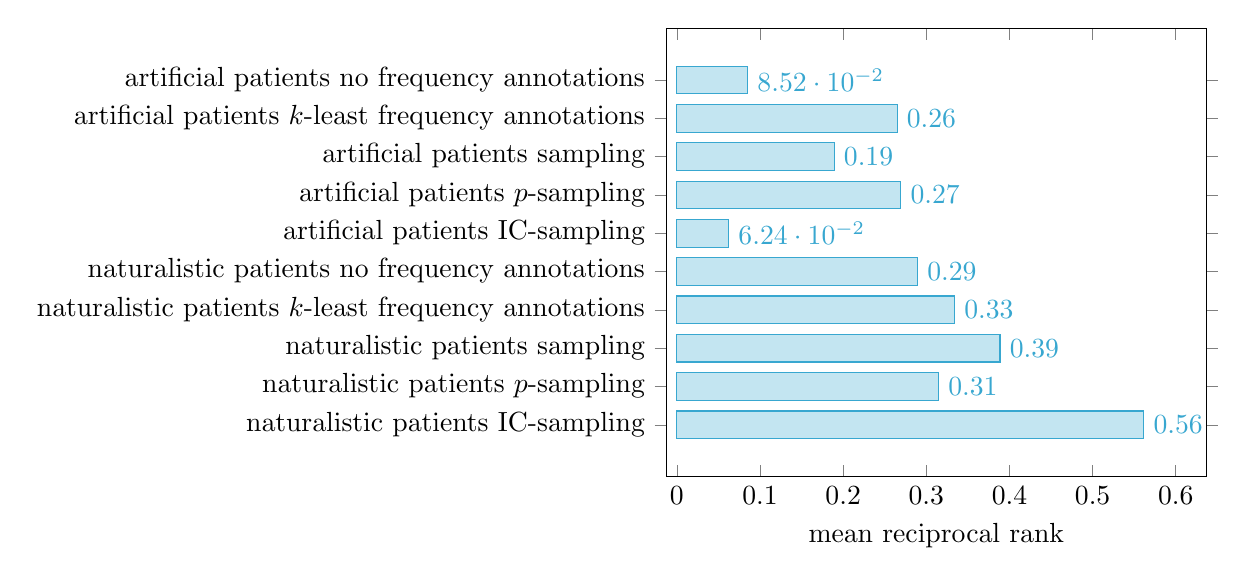
\begin{tikzpicture}
        \begin{axis}[
            xbar,
            enlargelimits=0.15,
            xlabel={mean reciprocal rank},
            symbolic y coords={
                % UPSIDE DOWN!
                naturalistic patients IC-sampling,
                naturalistic patients $p$-sampling,
                naturalistic patients sampling,
                naturalistic patients $k$-least frequency annotations,
                naturalistic patients no frequency annotations,
                artificial patients IC-sampling,
                artificial patients $p$-sampling,
                artificial patients sampling,
                artificial patients $k$-least frequency annotations,
                artificial patients no frequency annotations,
            },
            ytick=data,
            nodes near coords, 
            nodes near coords align={horizontal},
            yticklabel style={text height=1.5ex}, % To make sure the text labels are nicely aligned
            ]
            \addplot coordinates{
                (0.0852059148701,artificial patients no frequency annotations)
                (0.264807383628,artificial patients $k$-least frequency annotations)
                (0.189174526493,artificial patients sampling)
                (0.269227574751,artificial patients $p$-sampling)
                (0.062358752126,artificial patients IC-sampling)
                (0.289438943894,naturalistic patients no frequency annotations)
                (0.333880427171,naturalistic patients $k$-least frequency annotations)
                (0.388596491228,naturalistic patients sampling)
                (0.314673913043,naturalistic patients $p$-sampling)
                (0.561606160616,naturalistic patients IC-sampling)
            };
        \end{axis}
    \end{tikzpicture}
    \label{fig:mrrgen}
    \caption{All diseases pooled.}
    \end{subfigure}
    
    \vspace{1cm}

    \begin{subfigure}{0.99\textwidth} \centering
    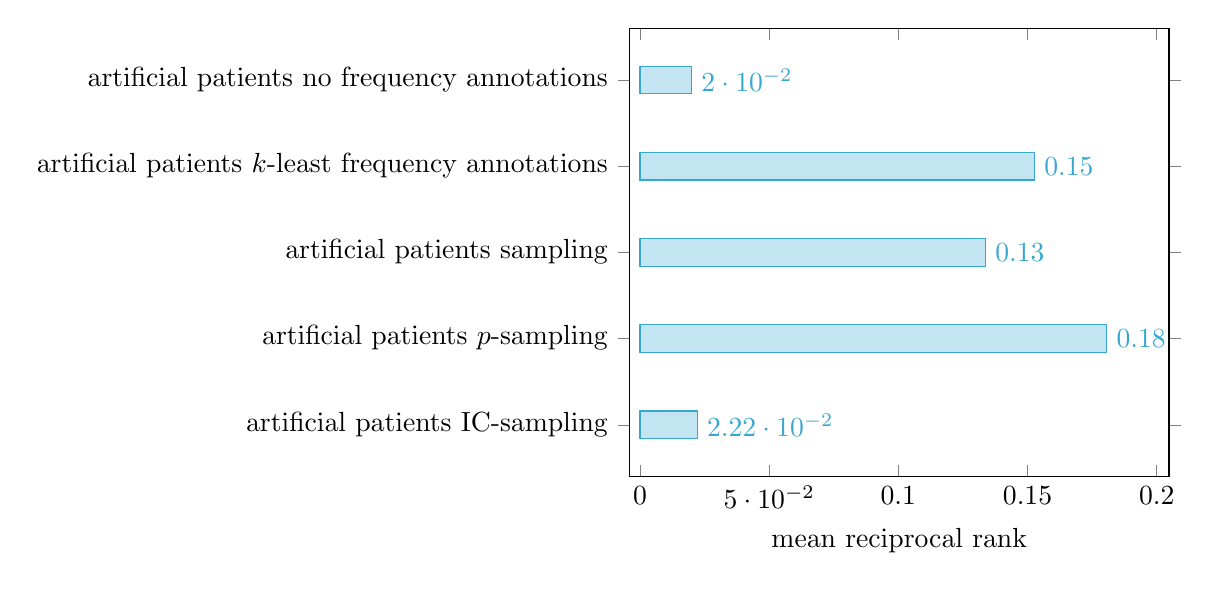
\begin{tikzpicture}
        \begin{axis}[
            xbar,
            enlargelimits=0.15,
            xlabel={mean reciprocal rank},
            symbolic y coords={
                % UPSIDE DOWN!
                artificial patients IC-sampling,
                artificial patients $p$-sampling,
                artificial patients sampling,
                artificial patients $k$-least frequency annotations,
                artificial patients no frequency annotations,
            },
            ytick=data,
            nodes near coords, 
            nodes near coords align={horizontal},
            yticklabel style={text height=1.5ex}, % To make sure the text labels are nicely aligned
            ]
            \addplot coordinates{
                (0.020012015728,artificial patients no frequency annotations)
                (0.152694351749,artificial patients $k$-least frequency annotations)
                (0.133770278138,artificial patients sampling)
                (0.180666666667,artificial patients $p$-sampling)
                (0.0221883556896,artificial patients IC-sampling)
            };
        \end{axis}
    \end{tikzpicture}
    \caption{Only diseases with negative annotations.}
    \label{fig:mrrneg}
    \end{subfigure}
    \caption{Mean reciprocal rank plots.}
    \label{fig:mrr}
\end{figure}

From the results in \Figure{fig:mrr}, we see an interesting pattern:
the models that perform relatively badly on the arificial data tend to perform well 
on the naturalistic data, according to this metric.
%
For example, the IC-sampling model performs worst on the artificial data, but performs
best on the naturalistic data.
%
The exception is the no-frequency model, which consistently performs badly, 
as to be expected because it is too simplistic.

\subsubsection{Binned rank counts}
\label{subsubsec:metricbrc}
%
To construct the binned rank plots,
we count the number of test cases for which the gold-standard disease falls into the
ranking bin of interest.

\begin{figure}[h]
    \begin{subfigure}{0.99\textwidth} \centering
    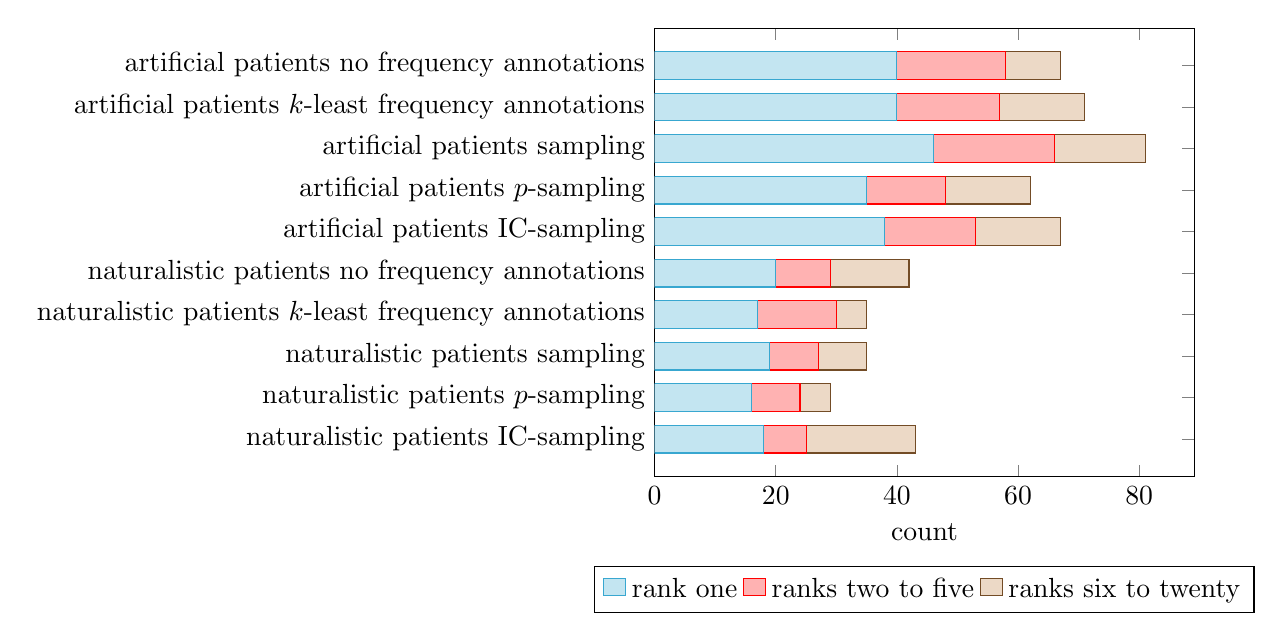
\begin{tikzpicture}
        \begin{axis}[
            xbar stacked,
            xlabel={count},
            xmin=0,
            legend style={at={(0.5,-0.20)}, anchor=north,legend columns=-1},
            symbolic y coords={
                % UPSIDE DOWN!
                naturalistic patients IC-sampling,
                naturalistic patients $p$-sampling,
                naturalistic patients sampling,
                naturalistic patients $k$-least frequency annotations,
                naturalistic patients no frequency annotations,
                artificial patients IC-sampling,
                artificial patients $p$-sampling,
                artificial patients sampling,
                artificial patients $k$-least frequency annotations,
                artificial patients no frequency annotations,
            },
            ytick=data,
            yticklabel style={text height=1.5ex}, % To make sure the text labels are nicely aligned
            ]
            \addplot coordinates{
                (40,artificial patients no frequency annotations)
                (40,artificial patients $k$-least frequency annotations)
                (46,artificial patients sampling)
                (35,artificial patients $p$-sampling)
                (38,artificial patients IC-sampling)
                (20,naturalistic patients no frequency annotations)
                (17,naturalistic patients $k$-least frequency annotations)
                (19,naturalistic patients sampling)
                (16,naturalistic patients $p$-sampling)
                (18,naturalistic patients IC-sampling)
            };
            \addlegendentry{rank one}
            \addplot coordinates{
                (18,artificial patients no frequency annotations)
                (17,artificial patients $k$-least frequency annotations)
                (20,artificial patients sampling)
                (13,artificial patients $p$-sampling)
                (15,artificial patients IC-sampling)
                (9 ,naturalistic patients no frequency annotations)
                (13,naturalistic patients $k$-least frequency annotations)
                (8 ,naturalistic patients sampling)
                (8 ,naturalistic patients $p$-sampling)
                (7 ,naturalistic patients IC-sampling)
            };
            \addlegendentry{ranks two to five}
            \addplot coordinates{
                (9 ,artificial patients no frequency annotations)
                (14,artificial patients $k$-least frequency annotations)
                (15,artificial patients sampling)
                (14,artificial patients $p$-sampling)
                (14,artificial patients IC-sampling)
                (13,naturalistic patients no frequency annotations)
                (5 ,naturalistic patients $k$-least frequency annotations)
                (8 ,naturalistic patients sampling)
                (5 ,naturalistic patients $p$-sampling)
                (18 ,naturalistic patients IC-sampling)
            };
            \addlegendentry{ranks six to twenty}
        \end{axis}
    \end{tikzpicture}
    \caption{Artificial and naturalistic patients; general disease.}
    \label{brc}
    \end{subfigure}
    
    \vspace{1cm}

    \begin{subfigure}{0.99\textwidth} \centering
    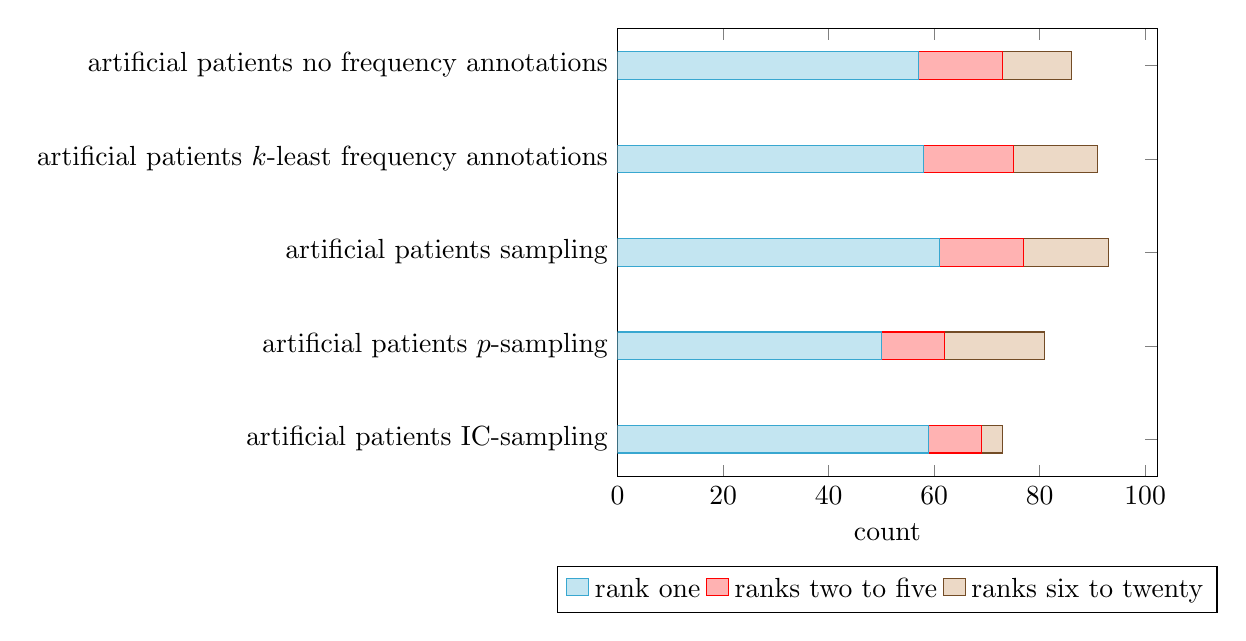
\begin{tikzpicture}
        \begin{axis}[
            xbar stacked,
            xlabel={count},
            xmin=0,
            legend style={at={(0.5,-0.20)}, anchor=north,legend columns=-1},
            symbolic y coords={
                % UPSIDE DOWN!
                artificial patients IC-sampling,
                artificial patients $p$-sampling,
                artificial patients sampling,
                artificial patients $k$-least frequency annotations,
                artificial patients no frequency annotations,
            },
            ytick=data,
            yticklabel style={text height=1.5ex}, % To make sure the text labels are nicely aligned
            ]
            \addplot coordinates{
                (57,artificial patients no frequency annotations)
                (58,artificial patients $k$-least frequency annotations)
                (61,artificial patients sampling)
                (50,artificial patients $p$-sampling)
                (59,artificial patients IC-sampling)
            };
            \addlegendentry{rank one}
            \addplot coordinates{
                (16,artificial patients no frequency annotations)
                (17,artificial patients $k$-least frequency annotations)
                (16,artificial patients sampling)
                (12,artificial patients $p$-sampling)
                (10,artificial patients IC-sampling)
            };
            \addlegendentry{ranks two to five}
            \addplot coordinates{
                (13,artificial patients no frequency annotations)
                (16,artificial patients $k$-least frequency annotations)
                (16,artificial patients sampling)
                (19,artificial patients $p$-sampling)
                (4,artificial patients IC-sampling)
            };
            \addlegendentry{ranks six to twenty}
        \end{axis}
    \end{tikzpicture}
    \caption{Artificial patients; disease with negative annotations.}
    \label{brc1}
    \end{subfigure}
    \caption{Binned ranking plots.}
\end{figure}

The results in \Figure{brc1} and \Figure{brc} show a similar trend to those described in
\Section{subsubsec:metricmrr}: models that tend to do well on the artificial data, do worse
on the naturalistic data and vice versa.
%
In particular, the IC-sampling model does best by a large margin on the naturalistic data,
but has very low performance on the artificial data.
%
The exception to the analogy to
\Section{subsubsec:metricmrr} is that the sampling method performs well in both 
artificial and naturalistic data scenarios.

\section{Discussion}
\label{sec:dis}

In the present study, we have no information on correlations between diseases.
%
In particular, our ranking evaluation metrics do not take into account the
relative severity of ranking particular diseases above the gold-standard disease.
%
However, in reality it may be the case that the model ranks a close variant
above the gold-standard disease, in which case the misclassification cost
incurred should be lesser than if an unrelated disease were higher ranked.
%
A further investigation is necessary to determine whether the relative
performance of the considered methods would change under such a cost metric.



\section{Conclusion}
\label{sec:conc}

Draw groundbreaking conclusions.


\newpage
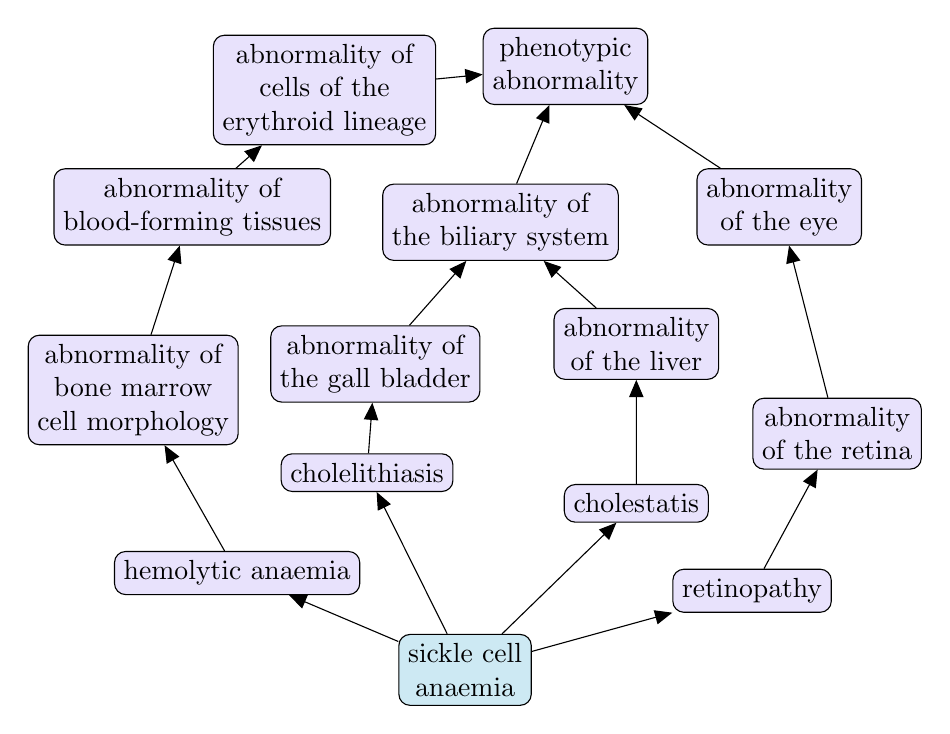
\begin{tikzpicture}[scale=0.15]
    \draw (39.9,-54.6) node[disease] (A) {sickle cell \\ anaemia};
    \draw (64.2,-47.9) node[phenotype] (B) {retinopathy};
    \draw (71.4,-34.6) node[phenotype] (C) {abnormality \\ of the retina};
    \draw (66.5,-15.4) node[phenotype] (D) {abnormality \\ of the eye};
    \draw (48.4,-3.5)  node[phenotype] (E) {phenotypic \\ abnormality};
    \draw (54.4,-40.5) node[phenotype] (F) {cholestatis};
    \draw (54.4,-27)   node[phenotype] (G) {abnormality \\ of the liver};
    \draw (42.9,-16.7) node[phenotype] (H) {abnormality of \\ the biliary system};
    \draw (31.6,-37.9) node[phenotype] (I) {cholelithiasis};
    \draw (32.3,-28.7) node[phenotype] (J) {abnormality of \\ the gall bladder};
    \draw (20.6,-46.4) node[phenotype] (K) {hemolytic anaemia};
    \draw (11.8,-30.9) node[phenotype] (L) {abnormality of \\ bone marrow \\ cell morphology};
    \draw (16.8,-15.4) node[phenotype] (M) {abnormality of \\ blood-forming tissues};
    \draw (28,-5.5)    node[phenotype] (N) {abnormality of \\ cells of the \\ erythroid lineage};
    \edge {A} {B};
    \edge {A} {F};
    \edge {A} {I};
    \edge {A} {K};
    \edge {B} {C};
    \edge {C} {D};
    \edge {D} {E};
    \edge {F} {G};
    \edge {G} {H};
    \edge {I} {J};
    \edge {J} {H};
    \edge {K} {L};
    \edge {L} {M};
    \edge {M} {N};
    \edge {N} {E};
    \edge {H} {E};
\end{tikzpicture}

\newcommand{\itemlayer}{$I_1$/A, $I_2$/B}
\newcommand{\hiddenquerylayers}{$H_1$/C/$Q_1$/J, $H_2$/D/$Q_2$/K, $H_3$/E/$Q_3$/L, $H_4$/F/$Q_4$/M, $H_5$/G/$Q_5$/N, $H_6$/H/$Q_6$/O, $H_7$/I/$Q_7$/P}

\begin{figure}[h]
    \begin{tikzpicture}
        \pgfmathsetmacro\diametersqr{1}
        \pgfmathsetmacro\rectwidth{2}
        \pgfmathsetmacro\rectheight{8}
        \pgfmathsetmacro\spacing{1}
        
        \pgfmathsetmacro\numnodesitem{2}
        \pgfmathsetmacro\numnodeshiddenquery{7}
        
        % item layer
        \xdef\xlist{4}
        \xdef\ylist{4}
        \pgfmathsetmacro\yoffset{\rectheight / \numnodesitem}
        \foreach \m/\n [count=\l] in \itemlayer{
            \foreach \k in {1,...,400}{ % try 400 times to place without a collision
                \pgfmathsetmacro\x{rnd*\rectwidth}
                \pgfmathsetmacro\y{(\l - 1)*\yoffset + rnd*\yoffset}
                \xdef\collision{0}
                \foreach \element [count=\i] in \xlist{
                    \pgfmathtruncatemacro\j{\i-1}
                    \pgfmathsetmacro\checkdistancesqr{ ( ({\xlist}[\j]-(\x))^2 + ({\ylist}[\j]-(\y))^2 ) }
                    \ifdim\checkdistancesqr pt<\diametersqr pt
                        \xdef\collision{1}
                        \breakforeach
                    \fi
                }
                \ifnum\collision=0
                    \xdef\xlist{\xlist,\x}
                    \xdef\ylist{\ylist,\y}
                    \draw (\x,\y) node[item on] (\n) {\m};
                    \breakforeach
                \fi 
            }
        }
        
        % hidden layer
        \xdef\xlist{4}
        \xdef\ylist{4}
        \pgfmathsetmacro\yoffset{\rectheight / \numnodeshiddenquery}
        \foreach \m/\n/\o/\p [count=\l] in \hiddenquerylayers{
            \foreach \k in {1,...,400}{ % try 400 times to place without a collision
                \pgfmathsetmacro\x{((-1)^\l)*rnd*\rectwidth + 2*\rectwidth + \spacing}
                \pgfmathsetmacro\y{(\l - 1)*\yoffset + rnd*\yoffset}
                \xdef\collision{0}
                \foreach \element [count=\i] in \xlist{
                    \pgfmathtruncatemacro\j{\i-1}
                    \pgfmathsetmacro\checkdistancesqr{ ( ({\xlist}[\j]-(\x))^2 + ({\ylist}[\j]-(\y))^2 ) }
                    \ifdim\checkdistancesqr pt<\diametersqr pt
                        \xdef\collision{1}
                        \breakforeach
                    \fi
                }
                \ifnum\collision=0
                    \xdef\xlist{\xlist,\x}
                    \xdef\ylist{\ylist,\y}
                    \draw (\x,\y) node[hidden on] (\n) {\m};
                
                    \pgfmathsetmacro\x{\x + 2*\rectwidth + \spacing}
                    \draw (\x,\y) node[query on] (\p) {\o};
                    
                    \breakforeach
                \fi 
            }
        }
        
        % edges from item to hidden layer
        \edge {A} {C,F};
        \edge {B} {H};
        
        % edges from hidden to query layer
        \edge {C} {J};
        \edge {D} {K};
        \edge {E} {L};
        \edge {F} {M};
        \edge {G} {N};
        \edge {H} {O};
        \edge {I} {P};
        
        % edges within hidden layer
        \edge {C} {E};
        \edge {D} {E};
        \edge {E} {F};
        \edge {F} {G};
        \edge {G} {I};
        \edge {H} {I};
        
        % edges within query layer
        \edge {L} {J};
        \edge {L} {K};
        \edge {M} {L};
        \edge {N} {M};
        \edge {P} {N};
        \edge {P} {O};
        
        % surrounding boxes
        \node (X) [draw=blue, fit= (A) (B), inner sep=0.2cm, ultra thick, fill=blue!20, fill opacity=0.2] {};
        \node [yshift=2.0ex] at (X.north) {\textbf{item layer}};
        
        \node (Y) [draw=orange, fit= (C) (D) (E) (F) (G) (H) (I), inner sep=0.2cm, ultra thick, fill=orange!20, fill opacity=0.2] {};
        \node [yshift=2.0ex] at (Y.north) {\textbf{hidden layer}};
        
        \node (Z) [draw=purple, fit= (J) (K) (L) (M) (N) (O) (P), inner sep=0.2cm, ultra thick, fill=purple!20, fill opacity=0.2] {};
        \node [yshift=2.0ex] at (Z.north) {\textbf{query layer}};
    \end{tikzpicture}
    \caption{BOQA network structure.\footnotemark}
\end{figure}
\footnotetext{Reproduced from \bibentry{bauer2012bayesian}.}











\newpage

\begingroup
    \captionsetup[figure]{name=Algorithm}
    \begin{figure}[h]
        \begin{algorithm}[caption={Integer division},label={alg1}]
    input: parameters $\displaystyle\alpha$, $\beta$, query $(q_1, \hdots, q_m)$
    $a \gets 0$
    foreach $i \in \{1, \hdots, n\}$
        foreach $j \in \{1, \hdots, m\}$
            if item $i$ is explicitly or implicitly annotated to term $j$
                $h_j \gets 1$
            else
                $h_j \gets 0$
        foreach $x, y \in \{0, 1\}$
            $m_{xy1 \mid QH} \gets  \left|  \left\{k \mid \left( q_k = x  \right) \wedge  \left( h_k = y \right) \right\} \right|$
        $a_i \gets \beta^{\,m_{011\mid QH}} \;(1 - \beta)^{m_{111\mid QH}} \;\alpha^{m_{001\mid QH}} \;(1 - \alpha)^{m_{101\mid QH}}$
        $a \gets a + a_i$
    foreach $i \in \{1, \hdots, n\}$ 
        $p_i \gets a_i/a$
    return $(p_1, \hdots, p_n)$
        \end{algorithm}
        \caption{MAP inference without frequency.\footnotemark}
    \end{figure}
\endgroup

\footnotetext{Reproduced from \bibentry{bauer2012bayesian}.}


\newpage
\bibliographystyle{plain}
\bibliography{project}

\end{document}
